\documentclass[refman]{article} 
\setcounter{tocdepth}{3}
\setcounter{secnumdepth}{4}
\usepackage{dirtree}
\usepackage{xcolor}
\usepackage{listings}
\usepackage[utf8]{inputenc}
\usepackage{hyperref}
\usepackage{amsmath}
\usepackage[a4paper, hmargin=2.54cm, vmargin=1.9cm]{geometry}
\usepackage{natbib}
\bibliographystyle{plain}
\usepackage{enumitem}

\usepackage{tikz}
\usetikzlibrary{shapes.geometric, arrows}
\tikzstyle{startstop} = [rectangle, rounded corners, minimum width=3cm, minimum height=1cm,text centered, draw=black, fill=red!30]
\tikzstyle{io} = [trapezium, trapezium left angle=70, trapezium right angle=110, minimum width=3cm, minimum height=1cm, text centered, draw=black, fill=blue!30]
\tikzstyle{process} = [rectangle, minimum width=3cm, minimum height=1cm, text centered, draw=black, fill=orange!30]
\tikzstyle{decision} = [diamond, minimum width=3cm, minimum height=1cm, text centered, draw=black, fill=green!30]
\tikzstyle{arrow} = [thick,->,>=stealth]



\definecolor{codegreen}{rgb}{0,0.6,0}
\definecolor{codegray}{rgb}{0.5,0.5,0.5}
\definecolor{codepurple}{rgb}{0.58,0,0.82}
\definecolor{backcolour}{rgb}{0.95,0.95,0.92}

\lstdefinestyle{mystyle}{
	backgroundcolor=\color{backcolour},   
	commentstyle=\color{codegreen},
	keywordstyle=\color{magenta},
	numberstyle=\tiny\color{codegray},
	stringstyle=\color{codepurple},
	basicstyle=\ttfamily\footnotesize,
	breakatwhitespace=false,         
	breaklines=true,                 
	captionpos=b,                    
	keepspaces=true,                 
	numbers=left,                    
	numbersep=5pt,                  
	showspaces=false,                
	showstringspaces=false,
	showtabs=false,                  
	tabsize=2
}

\lstset{style=mystyle}


\title{Cryptocurrency Orderbook Analysis Tool}
\author{Ivan E. Perez}
\date{\today\\v1.0.2}
\begin{document} 
\maketitle
\pagenumbering{roman} 
\tableofcontents 

 
\pagenumbering{arabic} 
\pagestyle{headings} 


\section{Introduction} 
This project is an extension of my thesis, <a \href{"https://academicworks.cuny.edu/cgi/viewcontent.cgi?article=1682&context=hc_sas_etds"}{ A Study of CUSUM Statistics on Bitcoin Transactions}, where I was tasked with implementing CUSUM statistic processes to identify price actions periods in bitcoin markets. After developing a tool for market orders, the natural extension was to find relationships from activities in the limit order book. I started developing this tool to record instances of the limit order book in order to record Limit Order insertions (LO), cancellations (CO), and Market Orders (MO).

As the project grew I wanted to make a tool that could be used by academics looking to apply and develop market microstructure models in live markets. As a result, the styles in which the limit orderbook and orderbook events are recorded are being developed in accordance to the conventions presented in recent market microstructure papers correspond to the following papers:
\begin{enumerate}
	\item \href{https://arxiv.org/pdf/1312.0563.pdf}{Huang W., Lehalle C.A. and Rosenbaum M. - Simulating and analyzing order book data:The queue-reactive model}\cite{Huang:2020}
	\item \href{https://citeseerx.ist.psu.edu/viewdoc/download?doi=10.1.1.139.1085&rep=rep1&type=pdf}{Cont R., Stoikov S. and Talreja R. - A stochastic model for order book dynamics}
	
	\item \href{https://arxiv.org/pdf/1011.6402.pdf}{Cont R., Kukanov A. and Stoikov S. - The price impact of order book events}
	
	\item \href{https://papers.ssrn.com/sol3/papers.cfm?abstract_id=3431139}{Cartea. A, Jaimungal S. and Wang Y. - Spoofing and Price Manipulation in Order Driven Markets}
	
	\item \href{https://link.springer.com/article/10.1007/s42521-019-00007-w#article-info}{Silyantev, E. - Order flow analysis of cryptocurrency markets}\footnote{This paper shows a working model implementing Order Flow Imbalance (OFI) and Trade Flow Imbalance(TFI) to BTC-USD trades was done by \href{https://medium.com/@eliquinox/order-flow-analysis-of-cryptocurrency-markets-b479a0216ad8}{Ed Silyantev}. He developed a tool to assess OFI and TFI of XBT-USD pair. }
\end{enumerate}

\newpage
\section{crobat Features} 

\subsection{Orderbook updating}
\begin{itemize}
	\item Order book recording module that maintains a time-series of:
	\begin{enumerate}
		\item Limit order insertions, cancellations and market orders,
		\item volumes at $n^{\textrm{th}}$ best limits, and
		\item prices at  $n^{\textrm{th}}$ best limits.
	\end{enumerate}
\end{itemize}

\newpage

\section{Getting Started and Installation}

\subsection{CoPrA}

\subsection{Installation}

Given that this is still very much a work in progress, it may make more sense to fork the project, or download the project as a compressed folder, and build \texttt{CSV\_out\_test.py} with your preferred settings.
\medskip
\hrule
\smallskip
\noindent \textbf{Note:} depending on the popularity of the asset and the computational power of your PC, you may run into errors arising from the computer not being able to keep up with the market (especially BTC-USD). I would suggest experimenting with an unpopular pair, (e.g.,  XRP-USD), or a crypto-crypto pair (e.g., XRP-BTC), and timing your queries outside of NYSE, and London Stock Exchange trading hours as they tend to have less activity.
\smallskip
\hrule
however if you want an easy installation: 

```pip3 install crobat``` 

\newpage

\section{Time-series Data Structure Layout}

\subsection{Introduction}


Since this is an orderbook <u>recorder</u> my use until now has been to record the orderbook. However there are accessors in the ```LOB\_funcs.py``` file, under in the *history* class. In the /test folder there is a small usecase if you would like to see it but documentation is pending.

1. For now we only have the full orderbook, with no regard for ticksize, and we call that ```recorder\_full.py```. 

2. We change the ```settings``` variable in the ```CSV\_out\_test.py``` file that has arguments for:

\begin{center}
	\begin{tabular}{|l|l|l|l|}
		\hline
		Parameter & Function Arg & Type/Format & Description \\
		\hline
		Recording Duration & \texttt{duration}& \texttt{int} & recording time in seconds\\
		Position Range & \texttt{position\_range} & \texttt{int} & ordinal distance from the best bid(ask)\\
		Currency Pair\footnote{\href{https://help.coinbase.com/en/pro/trading-and-funding/cryptocurrency-trading-pairs/locations-and-trading-pairs}{List of currency pairs supported by Coinbase}} & \texttt{currency\_pair} & \texttt{str} &\\
		\hline
	\end{tabular}
	
\end{center}

%| Parameter                | Function Arg  | Type |  Description | 
%|-------------------------|-------------------|------| -------|
%| Recording Duration | duration      | int  | recording time in seconds | 
%| Position Range     | position_range| int  | ordinal distance from the best bid(ask) |
%| Currency Pair      | currency_pair | str  | [List of currency pairs supported by Coinbase](https://help.coinbase.com/en/pro/trading-and-funding/cryptocurrency-trading-pairs/locations-and-trading-pairs) |

3. When you are ready, you can start the build. When it finishes you should get a message ```Connection Closed``` from ```CoPrA```. And the files for the limit orderbook for each side should be created with a timestamp:

%|Filename|side|description|
%|----|----|----|
%|L2_orderbook_events_askYYYY-MM-DDTHH:MM:SS.ffffff| ask|Time series of order book events on the ask side|
%|L2_orderbook_events_bidYYYY-MM-DDTHH:MM:SS.ffffff| bid| Time series of order book events on the bid side |
%|L2_orderbook_events_signedYYYY-MM-DDTHH:MM:SS.ffffff| both | Time series of order book events on both sides, - sign for bid, +sign for ask|
%|L2_orderbook_ask_volmYYYY-MM-DDTHH:MM:SS.ffffff| ask |Time series of the volume snapshots of order book on the ask side |
%|L2_orderbook_bid_volmYYYY-MM-DDTHH:MM:SS.ffffff| bid |Time series of the volume snapshots of order book on the bid side |
%|L2_orderbook_signed_volmYYYY-MM-DDTHH:MM:SS.ffffff | both |Time series of the volume  snapshots of the signed order book, - for bid, + for ask|
%|L2_orderbook_ask_volmYYYY-MM-DDTHH:MM:SS.ffffff| ask |Time series of the price snapshots of order book on the ask side |
%|L2_orderbook_bid_volmYYYY-MM-DDTHH:MM:SS.ffffff| bid |Time series of the price snapshots of order book on the bid side |
%|L2_orderbook_signed_volmYYYY-MM-DDTHH:MM:SS.ffffff | both |Time series of the price snapshots of the signed order book, - for bid, + for ask|

\subsection{Understanding The Raw Order Book Data}

The coinbase exchange operates using the double auction model, the \href{https://docs.pro.coinbase.com/}{Coinbase Pro API}, and by extension the \href{https://copra.readthedocs.io/en/latest/}{CoPrA API} makes it relatively easy to get still images of an instance of the orderbook as \href{(https://docs.pro.coinbase.com/#the-level2-channel)}{\texttt{snapshots}} and it sends updates in real time of the volume at a particular price level as \href{https://docs.pro.coinbase.com/#the-level2-channel}{\texttt{l2\_update}} messages. If you would like to know more, the cited papers do a great job introducing the double auction model for the purposes of defining the types of orders, and how they record events and make sense of them. 

\subsubsection{Order Book Snapshots}

Below there is a graph of the snapshot where bids (green) show open limit orders to buy the 1 unit of the cryptocurrency below \$7085.930, and asks (red) show open limit orders to buy 1 unit above \$7085.930. The x-axis shows the price points, and the y-axis is the aggregate size at the price level. Note that  the signed order book calls volume on the bid side negative. 

%<img src="https://raw.githubusercontent.com/orderbooktools/crobat/master/images/figure_1.png" >

Early and current works relied on exchanges and private data providers (e.g., \href{https://data.nasdaq.com/BookViewer.aspx}{NASDAQ - BookViewer},\href{https://lobsterdata.com/}{LOBSTER} to provide reconstructions of order books. Earlier works were limited to taking snapshots and inferring the possible sequence of order book events between states. Coinbase and by extension crobat update the levels on the instance of a update message from the exchange so there is no guess as to what happened between states of the order book. The current format of the order book snapshot is not aggregated. The format of the order book snapshot for a single side is shown below

\begin{center}
	\begin{tabular}{|l|l|}
		\hline
		Item & Description/Format \\
		\hline
		Timestamp & YYYY-MM-DDTHH:MM:SS.ffffff\\ $1$ & total BTC at position 1 \\
		$2$ &total BTC at position 1 \\
		$\ldots$ & \ldots \\
		$n$ & total BTC at position n \\
		\hline
	\end{tabular}
\end{center}

\textbf{Incl. sample output of an entry}

The associated price quote (price quote (USD per XTC))snapshot is also generated, to make generation of market depth feasible. 

\begin{center}
	\begin{tabular}{|l|l|}
		\hline
		Item & Description/Format \\
		\hline
		Timestamp & YYYY-MM-DDTHH:MM:SS.ffffff\\ 
		$1$ & price quote at position 1 \\
		$2$ &price quote at position 1 \\
		$\ldots$ & \ldots \\
		$n$ & price quote at position n \\
		\hline
	\end{tabular}
\end{center}


Event recording are a timeseries of MO, LO, CO's as afforded from the \texttt{l2\_update} messages which are used to update the price, volume pair size at each price level. The format of the Event recorder is as follows:

\begin{center}
	
	\begin{tabular}{|l|l|l|}
		\hline
		Item & Description & format \\
		\hline
		Timestamp & Timestamp of when the event occurred &  YYYY-MM-DDTHH:MM:SS.ffffff\\
		order type & MO, LO, CO & \texttt{str} $\in \left\{\texttt{`market',`limit', `cancellation'}\right\}$\\
		price level & price of event occurrence in quote currency & \texttt{float64}\\
		event size & size of event in base currency\footnote{given constraints on the tick size of quote currency (e.g., USD =: \$0.01) we round the event size to the nearest decimal that would correspond to a move constrained by the minimum tick size.} & \texttt{float64}\\
		position & signed position (-- for bids, + for asks) & \texttt{int}\\
		mid price & (best-ask + best-bid)/2 & \texttt{float64}\\
		spread & best-ask + best-bid & \texttt{float64}\\
		\hline
	\end{tabular}
\end{center}

\subsubsection{Signed Order Book}
\paragraph{Signed Order Book Snapshot Prices}
The signed orderbook takes a different approach to position labelling so please keep that in mind. (note: I should  shift the position index to start at 1, for singe side order book snapshot time series). The signed orderbook snapshot is generated in a similar fashion with a volume, and price at each position. However, it uses the convention established in [3] for the signed order book. where positions on the bid are negative, with negative volume (XTC). I'll show the default setting that displays the 5 best bids and asks on each side.

\begin{center}
	\begin{tabular}{|l|l|}
		\hline
		Item & Description/Format \\
		\hline
		Timestamp & YYYY-MM-DDTHH:MM:SS.ffffff\\ 
		$-n$ & price quote at the $n^{\text{th}}$ best bid (i.e., worst bid) \\
		$-n+1$ & aggregate XTC limit buys at the second to worst bid \\
		$\ldots$ & \ldots \\
		$-2$ & aggregate XTC being bid for at the $2^{nd}$ best bid \\
		$-1$ & aggregate XTC limit being bid for at the best bed bid \\
		$1$ & aggregate XTC offered at the best ask\\
		$2$ & aggregate XTC offered at the $2^{\text{nd}}$ best ask\\
		\ldots & \ldots \\
		$n-1$ & aggregate XTC offered at the second worst ask \\
		$n$ & aggregate XTC offered at the worst ask \\
		\hline
	\end{tabular}
\end{center}


Similar to the single side implementation, there is an associated price quote  (e.g., USD per XTC) snapshot generated at each timepoint. The default format is given below:

\begin{center}
	\begin{tabular}{|l|l|}
		\hline
		Item & Description/Format \\
		\hline
		Timestamp & YYYY-MM-DDTHH:MM:SS.ffffff\\ $-n$ & price quote at the $n^{\text{th}}$ best bid (i.e., worst bid) \\
		$-n+1$ & price quote at the second to worst bid \\
		$\ldots$ & \ldots \\
		$-2$ & price quote at the $2^{nd}$ best bid \\
		$-1$ & price quote at the best bed bid \\
		$1$ & price quote at the best ask\\
		$2$ & price quote at the $2^{\text{nd}}$ best ask\\
		\ldots & \ldots \\
		$n-1$ & price quote at the second worst ask \\
		$n$ & price quote at the worst ask \\
		\hline
	\end{tabular}
\end{center}

\paragraph{Signed Events}

\medskip
\noindent Signed event recordings follow the convention from \href{https://arxiv.org/pdf/1011.6402.pdf}{The Price impact of Orderbook events}, where positive order flow is due to MO's on the buy side, CO on the sell side, and LO on the buy side. Conversely,  negative order flow is due to MO's on the sell side, CO on the buy side, and LO on the buy side. The format is similar to the single side order book events time-series, but the order volume is signed based on the aforementioned construction. 

\begin{center}
	
	\begin{tabular}{|l|l|l|}
		\hline
		Item & Description & format \\
		\hline
		Timestamp & Timestamp of when the event occurred &  YYYY-MM-DDTHH:MM:SS.ffffff\\
		order type & MO, LO, CO & \texttt{str} $\in \left\{\texttt{`market',`limit', `cancellation'}\right\}$\\
		price level & price of event occurrence in quote currency & \texttt{float64}\\
		event size & size of event in base currency\footnote{given constraints on the tick size of quote currency (e.g., USD =: \$0.01) we round the event size to the nearest decimal that would correspond to a move constrained by the minimum tick size.} & \texttt{float64}\\
		position & signed position (-- for bids, + for asks) & \texttt{int}\\
		side & bid/ask side where the event occurs & \texttt{str} $\in \left\{\texttt{`buy',`sell'}\right\}$\\
		mid price & (best-ask + best-bid)/2 & \texttt{float64}\\
		spread & best-ask + best-bid & \texttt{float64}\\
		\hline
	\end{tabular}
	
\end{center}

\subsection{Final notes on Orderbook interpretation}

write about how the program object sees the orderbook with an example of code. 


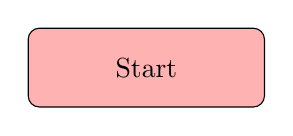
\begin{tikzpicture}[node distance=2cm]
	\node (start) [startstop] {Start};
\end{tikzpicture}


\newpage

\section{Modules}
	The module dependency of the program are organized as follows:
	\dirtree{%
		.1 CSV\_out\_test.py.
		.2 recorder\_full.py.
		.3 asyncio, time.
		.3 dateime.
		.3 copra.websocket.
		.3 pandas(note can move this later).
		.3 LOB\_funcs.py.
		.4 pandas.
		.4 copy.
		.4 bisect.
		.4 numpy.
		.4 history\_funcs.py.
		.3 history\_funcs.py.
		.4 pandas.
		.4 bisect.
		.3 gc.
		.3 numpy.
		.2 datetime.
		.2 copra.rest.
		.2 copra.websocket.
	}


	\subsection{recorder\_full}
	
	\subsubsection{Description}
	
	The \texttt{recorder\_full} module contains the class \textcolor{olive}{\texttt{L2\_Update}}. \textcolor{olive}{\texttt{L2\_Update}} is responsible for:
	\begin{itemize}
		\item initializing instances of the order book history class, \textcolor{olive}{\texttt{history}}.
		\item interpreting the snapshot, ticker and l2update messages that come from the websocket.
		\item calling the appropriate functions and classes to carry out the orderly update to the limit order book, and order book history arrays.
	\end{itemize}

	\subsubsection{\textit{Class} \textcolor{olive}{\texttt{L2\_Update}} }
	
	\textbf{Function list}:
	\begin{itemize}
		\item \textcolor{blue}{\texttt{\_\_init\_\_}}\texttt{(self, loop, channel, input\_args)}
		\item
		\textcolor{blue}{\texttt{on\_open}}\texttt{(self)}
		\item \textcolor{blue}{\texttt{on\_message}}\texttt{(self, msg)}
		\item \textcolor{blue}{\texttt{on\_close}}\texttt{(self, was\_clean, code, reason)}
	\end{itemize}

	\textcolor{blue}{\texttt{\_\_init\_\_}}\texttt{(self, loop, channel, input\_args)}
	\medskip
	
	\noindent \textbf{Description:} Inheriting attributes \texttt{loop}, and \texttt{channel}, from \textcolor{olive}{\texttt{Client}}, it
	\begin{enumerate} 
		\item initializes the class \texttt{history} imported from \texttt{LOB\_funcs} and
		\item passes on the settings from the class \texttt{input\_args} and \item uses functions \textcolor{blue}{\texttt{on\_message}}\texttt{(self, msg)},
		\item \textcolor{blue}{\texttt{on\_close}}\texttt{(self, was\_clean, code, reason)} to manage incoming messages.
	\end{enumerate} 


	

\paragraph{\textit{function} \textcolor{blue}{\texttt{\_\_init\_\_}}\texttt{(self, loop, channel, input\_args)}}\hfill\break
\noindent \textbf{Description:} Initializes the class, using the attributes \texttt{loop, channel} from \texttt{Client} and attributes \texttt{position\_range, recording\_duration} from the class \texttt{input\_args}. It also creates an instance of the class \texttt{history}. 

\begin{tabular}{c r l }
	\textbf{parameters:}	& loop: & object\\
	&  & Comes from CoPrA\\
	&channel:& object\\
	&&comes from CoPrA\\
	&input\_args:& class\\
	&& passes on arguments for recording duration, and position range	
\end{tabular}

\begin{tabular}{l c l}
	\textbf{returns:} & None & \\
\end{tabular}

\textbf{Example: None}
%	\begin{lstlisting}[language=Python, caption=Python example]
%	 	settings = input\_args (recording_duration=5, position_range=5)
%	 	
%	 	channel1 = Channel()
%	 	channel2 = 
%	 	def hellobaby(self, yo, mama)
%	 \end{lstlisting}

	\paragraph{\textit{function} \textcolor{blue}{\texttt{on\_open}}\texttt{(self)}}
\hfill\break
\textbf{Description:} From class \texttt{Client} uses method \texttt{on\_open}\texttt{()} to set things up. See ACoPrA \texttt{on\_open()} for more information.

\noindent \textit{restated from} \texttt{CoPrA}:\hfill\break
\fbox{\begin{minipage}{\textwidth}
		\texttt{on\_open} is called as soon as the initial WebSocket opening handshake is complete. The connection is open, but the client is not yet subscribed.
		
		If you override this method it is important that you still call it from your subclass’ \texttt{on\_open} method, since the parent method sends the initial subscription request to the WebSocket server. Somewhere in your \texttt{on\_open} method you should have \texttt{super().on\_open()}.
		
		In addition to sending the subscription request, this method also logs that the connection was opened.
\end{minipage}}

\textbf{paramters:} None

\textbf{returns:} None
	
	\paragraph{\textit{function} \textcolor{blue}{\texttt{on\_message}}\texttt{(self, msg)},}
\hfill\break
\textbf{Description:} 
After matching \texttt{msg['type']} to \texttt{'snapshot','ticker', 'l2update'} do one of three actions,
\begin{center}
	\begin{tabular}{ |c|c| }
		\hline
		\texttt{msg['type'] ==} & action\\
		\hline
		\texttt{'snapshot'}&initialize the limit order book using the \texttt{initialize\_snap\_events}\\
		\hline
		\texttt{'ticker'}&  parse a market order,\\
		\hline
		\texttt{'l2update'}& parse a limit order insertion or cancellation to the limit order book.\\
		\hline
	\end{tabular}
\end{center}

\noindent \textit{restated from} \texttt{CoPrA}:\hfill\break
\fbox{\begin{minipage}{\textwidth}
		\texttt{on\_message}on is called every time a message is received. message is a dict representing the message. Its content will depend on the type of message, the channels subscribed to, etc. Please read Coinbase Pro’s WebSocket API documentation to learn about these message formats.
		
		Note that with the exception of errors, every other message triggers this method including things like subscription confirmations. Your code should be prepared to handle unexpected messages.
		
		This default method just prints the message received. If you override this method, there is no need to call the parent method from your subclass’ method.
\end{minipage}}

\begin{lstlisting}[language=Python, caption=Python example]
	class zepelli(object):
	def hellobaby(self, yo, mama)
\end{lstlisting}
%\begin{lstlisting}[language=Python, caption=Python example]
\textbf{Receiving a snapshot}:
\begin{enumerate}
	\item set the time to now UTC
	\item initialize the order book snapshots using self.
\end{enumerate}

	
	\paragraph{\textit{function} \textcolor{blue}{\texttt{on\_close}}\texttt{(self, was\_clean, code, reason)}}\hfill\break
\noindent \textbf{description:} The function called when the \texttt{close()} task is executed. Begins the post processing of accumulated time-series using the functions:
\begin{itemize}
	\item \texttt{hf.}\textcolor{blue}{\texttt{convert\_array\_to\_list\_dict}}
	\item \texttt{hf.}\textcolor{blue}{\texttt{convert\_array\_to\_list\_dict\_sob}}
	\item \texttt{hf.}\textcolor{blue}{\texttt{pd\_excel\_save}}
\end{itemize}

and \texttt{gc.}\textcolor{blue}{\texttt{collect()}} to clear memory after storing \texttt{.xlsx} files of the processed data.

\noindent \textit{restated from} \texttt{CoPrA}:\hfill\break
\fbox{\begin{minipage}{\textwidth}
		\texttt{on\_close} is called whenever the connection between the client and server is closed. \texttt{was\_clean} is a boolean indicating whether or not the connection was cleanly closed. code, an integer, and reason, a string, are sent by the end that initiated closing the connection.
		
		If the client did not initiate this closure and \texttt{client.auto\_reconnect} is set to True, the client will attempt to reconnect to the server and resubscribe to the channels it was subscribed to when the connection was closed. This method also logs the closure.
		
		If your subclass overrides this method, it is important that the subclass method calls the parent method if you want to preserve the auto reconnect functionality. This can be done by including \texttt{super().on\_close(was\_clean, code, reason)} in your subclass method.	
\end{minipage}}

\begin{tabular}{r r l }
	\textbf{parameters:}	& was\_clean:& bool \\
	& code: & int or None \\
	& reason: & str or None
\end{tabular}

\begin{tabular}{r r l}
	\textbf{returns:} & None: & None\\
\end{tabular}

\begin{lstlisting}[language=Python, caption=Python example]]
	# Needs an Example
\end{lstlisting}
	 
 

\subsection{LOBF\_funcs}
\hfill \break
\textbf{Description:} module that houses the class \texttt{history} and the methods that outline how to update snapshots.

\subsubsection{\textit{class} \texttt{history()}}\hfill \break
\textbf{Description:} Contains attributes for the time series array of the limit order book, the current snapshot of the limit order book and the time-series of the events in the limit order book. We detail the role of each attribute in the Table whateever. The class contains methods that operate of these attributes, in order to update the order book and record changes. The functions \texttt{UpdateSnapshot\_bid\_Seq} and \texttt{UpdateSnapshot\_ask\_Seq}found outside ofthese methods, dictate the sequence in which the methods contained in \texttt{history} are executed.

\paragraph{\textit{function} \textcolor{blue}{\texttt{\_\_init\_\_}}\texttt{(self)}}\hfill\break
\textbf{Description:} Initializes the lists and variables that will be operated on by other class methods. Each side, bid, ask and the combined signed has a list demarked by \texttt{\_history}, that will be populated by timestamped states of the limit order book. The lists prefixed by \texttt{snapshot} are populated by the state of limit order book demarked by the suffix \texttt{bid}, \texttt{ ask}, and \texttt{signed}. The variables \texttt{order\_type},  \texttt{position} and \texttt{event\_size} denote the type, position and size of the event based on the change in the order book as a result of an \texttt{l2\_update} message. The \texttt{token} variable determines whether the change in the order book is recorded in the events list. 
%
%\begin{itemize}
%	\item  bid\_history - list containing timeseries entries for the bid side in the form \texttt{[timestamp, snapshot\_bid]}
%	\item  ask\_history - list containing timeseries entries for the ask side in the form \texttt{[timestamp, snapshot\_ask]}
%	\item  signed\_history - list containing timeseries entries for the signed order book in the form \texttt{[timestamp, snapshot\_signed]}
%	\item snapshot\_bid - list containing current state of the order book on the bid side in the form \texttt{[[price, volm], \ldots ]}
%	\item snapshot\_bid - list containing current state of the order book on the bid side in the form \texttt{[[price, volm], \ldots ]}
%	\item snapshot\_bid - list containing current state of the order book on the bid side in the form \texttt{[[price, volm], \ldots ]}
%	\item order\_type 
%	\item token
%	\item position
%	\item event\_size 
%\end{itemize}

\begin{tabular}{r r l }
	\textbf{parameters:}	& None: & None\\
\end{tabular}

\begin{tabular}{r r l}
	\textbf{returns:} & None: & None\\
\end{tabular}

\textbf{Example: None}

\paragraph{initialize\_snap\_events}\hfill\break
\noindent\textbf{Description:} Method that parses the \texttt{snapshot}. Add the first entry to the collection of \_history variables. 

\textbf{function dependency:}
\begin{itemize}
	\item np.round
	\item hf.min\_dec
\end{itemize}
	
\paragraph{add\_market\_order\_message}
\hfill\break
\textbf{Description:}function that parses a message object, aggregates for duplicate timestamps, and appends them to the events list. 

\paragraph{remove\_price\_level()}
\hfill \break
\textbf{Description:} Checks the level depth of an l2\_update message, removes the existing price level from the snapshot array if the level depth is 0. 
counts as a change to the limit order book therefore self.token is set to True.

\textbf{returns} an updated snapshot 

\paragraph{update\_price\_level()}
\hfill \break
\textbf{Descirption:} updates the existing price level to a new size. Sets self.order type to insertion if the new size is larger than the old size, or cancellation if the new size is smaller than the old size. sets the position to the self.position variable to the index where this event happened.

\textbf{returns} an updated snapshot

%\paragraph{\textit{function} \textcolor{blue}{\texttt{update\_price\_index\_buy}}\texttt{(self, level\_depth, price\_level, pre\_level\_depth)}}\hfill\break
\noindent \textbf{Description:} If there is a new price level introduced, this function determines its location and appropriately inserts it into the snapshot bid array. It will also set the position, and token depending on where the change occurs. 

\begin{tabular}{r r l }
	\textbf{parameters:}	& level\_depth: & float64\\
	&  & level depth received from the \texttt{l2update} message\\
	& price\_level:& float64\\
	&& The price level being introduced\\
	& pre\_level\_depth:& float64\\
	&& some pre\_level\_depth that is reset to 0, idk this feature
\end{tabular}

\begin{tabular}{l c l}
	\textbf{returns:} & snapshot\_bid & list\\
	& & The modified snapshot\_bid.\\
	& bid\_range: & list \\
	&& The modified range of bids available in the snapshot.\\
	&pre\_level\_depth &float64\\
	&& again the pre level depth that idk why i still have this.\\
\end{tabular}

\textbf{Example: None}
\begin{lstlisting}[language=Python]
	x = __my_function__(1.234, True, 3)
	>>print(x)
	>>-1.23
	
	x = __my_function__(1.234, False, 3)
	>>print(x)
	>>1.23
\end{lstlisting}



\paragraph{update\_price\_index\_buy}\hfill\break 
\noindent\textbf{Description:}


\subsection{history\_funcs.py}\hfill \break
\noindent \textbf{Description}



\paragraph{\textbf{function} check\_order(snapshot, side)}\hfill\break
\noindent \textbf{Description}

\noindent \textbf{inputs}

\noindent \textbf{returns}

\paragraph{\textbf{function} convert\_array\_to\_list\_dict()}\hfill\break
\noindent \textbf{Description}

\textbf{inputs}
\textbf{returns}

\paragraph{\textbf{function} convert\_array\_to\_list\_dict\_sob()}\hfill\
\noindent \textbf{Description}

\textbf{inputs}
\textbf{returns}

\paragraph{\textbf{function} pd\_excel\_save()}\hfill\break
\noindent \textbf{Description}

\textbf{inputs}
\textbf{returns}

\paragraph{\textbf{function} set\_sign}\hfill\break
\noindent \textbf{Description}

\textbf{inputs}
\textbf{returns}

\paragraph{\textbf{function} set\_signed\_position}\hfill\break
\noindent \textbf{Description}

\textbf{inputs}
\textbf{returns}

\paragraph{\textbf{function} get\_min\_dec()}\hfill\break
\noindent \textbf{Description}

\textbf{inputs}
\textbf{returns}

\paragraph{\textbf{function} convert\_array\_to\_list\_dict\_sob()}\hfill\break
\noindent \textbf{Description}

\textbf{inputs}
\textbf{returns}

\newpage
\section{Contributing}
\subsection{Types of Contributions}
\subsubsection{Report Bugs}
Report bugs at \href{https://github.com/orderbooktools/crobat/issues}{https://github.com/orderbooktools/crobat/issues}
 
 If you are reporting a bug, please include:
 \begin{itemize}
 	\item Your operating system and version, or virtual environment setup
 	\item Details about the setup or container you might be using.
 	\item Detailed steps to reproduce the bug
 \end{itemize}
 
 \subsubsection{Fix Bugs}
 
 If you see something you can tackle in \href{https://github.com/orderbooktools/crobat/issues}{Issues}, if it is just a response or work around have at it. If you would like to fork the repository and fix it on your own, please do. When you attempt to merge it would be nice to get an email about it so I can also learn about the mistake. 
 
 \subsubsection{Implement Features}
 
 I will usually actively work on features for crobat. If somebody wants a particular feature it can be brought up in \href{https://github.com/orderbooktools/crobat/issues}{Issues.}
 \smallskip
 
 \noindent I will say the side project is implementing some features that report real-time statistics for changes in the order book.
 
 \subsubsection{Write Documentation}
 
 crobat could always use more documentation. For the manual I write in \LaTeX, (mostly because  I could not figure out PanDoc or Sphinx). If you write in either PanDoc or Sphinx and are interested in contributing significantly do not hesitate to contact me and I will try to learn how to convert this \texttt{.tex} file into a proper documentation repository.
 
 \subsubsection{Submit Feedback}
 
 Please submit feedback by filing an issue at:
 
 \noindent  \href{https://github.com/orderbooktools/crobat/issues}{https://github.com/orderbooktools/crobat/issues}.
 \smallskip
 
 \noindent If you are proposing a feature:\begin{itemize}
 	\item Explain in detail how it would work.
 	\item Keep the scope as narrow as possible, to make implementation feasible.
 	\item Remember that as an order book analysis tool for messages that arrive microseconds apart, we are very constrained in complexity of operations.
 	\item Since this a volunteer project, contributions are welcome.
 \end{itemize}
  
 \subsection{Getting Started!}
 I am not well versed in GitHub for starters. The way I make changes is:
 \begin{enumerate}
 	\item Make a clone of the directory and all the files of the package. 
 	\item Make changes on the file that I was working on.
 	\item Go through the PyPi package distribution wizard.
 	\item Compress the new package into a tarball.
 	\item Upload, and change files on the GitHub project page directory manually.
 	\item Flag the change in the GitHub change-log as a new release.
 \end{enumerate}

\noindent For you to contribute, I would fork the repository, then you can make changes on your forked repository on your own, and ask to merge to the main repository. I will then review and either accept or reject changes. I might ask you questions over email. 
 \newpage
 \section{Credits}
 \subsection{Development Lead}
 \begin{itemize}
 	\item Ivan E. Perez -  \href{mailto:perez.ivan.e@gmail.com}{perez.ivan.e@gmail.com}
 \end{itemize}
 \subsection{Contributors}
 \begin{itemize}
 	\item BTC-DAVE - \href{mailto:jewmansown69@gmail.com}{jewmansown69@gmail.com}
 \end{itemize}
 \newpage
 
  \section{License}
\noindent GNU GPLv3 License

\medskip
\noindent Copyright (c) 2020, Ivan E. Perez

\medskip
\noindent This program is free software: you can redistribute it and/or modify
it under the terms of the GNU General Public License as published by
the Free Software Foundation, either version 3 of the License, or
(at your option) any later version.
\smallskip
\noindent This program is distributed in the hope that it will be useful,
but WITHOUT ANY WARRANTY; without even the implied warranty of
MERCHANTABILITY or FITNESS FOR A PARTICULAR PURPOSE.  See the
GNU General Public License for more details.
\smallskip

\noindent You should have received a copy of the GNU General Public License
along with this program.  If not, see \href{https://www.gnu.org/licenses/}{https://www.gnu.org/licenses/}.

\section{History}
\subsection{0.0.2} 
\begin{itemize}
	\item First release on pypi.org
	\item Had to correct markdown formatting from YANKED 0.0.1 
\end{itemize}

\subsection{1.0.1}
\begin{itemize}
	\item Restructured order book so that the position index starts at 1.
	\item Added signed order book.
	\item Added output for the time series of order book prices and volumes.
	\item Simplified some queue update logic. 
\end{itemize}
\newpage
\section{Python Function Index}


 \section{Index}
 \section{To do list}
 \begin{enumerate}
 	\item daily goals
 	\begin{enumerate}
 		\item write 2 whole function definitions with description, examples, i/o, 
 		\item help format or rewrite one unique section. 
 	\end{enumerate}
 \end{enumerate}
%%%%%%%%%%%%%%%%%%%%%%%%%%%%%%%%%%%%%%%%%
%%                                     %%
%% Function Documentation Template     %%
%%									   %%
%%%%%%%%%%%%%%%%%%%%%%%%%%%%%%%%%%%%%%%%%


%%% DESCRIPTION %%%%
%%% Template to create function documentation in latex
%%% Follows a similar style to the documentation style in the python package Pandas 

\paragraph{\textit{function} \textcolor{blue}{\texttt{\_\_my\_function\_\_}}\texttt{(self, param\_1, param\_2=False, param\_3)}}\hfill\break
\noindent \textbf{Description:} Put your description here. In the next table we will state the parameters, on the left, with the object type on the right. just below it on the next line, we will give a brief description of the input parameter. After that we will use the returns portion in the exact same way. The final section is an example that uses \texttt{lstlisting} package to write snippets of python code for us. The filled out template is then included in the class .tex file and the class .tex file is included in the master manual .tex file.

For example this function will convert \texttt{param\_1} as a float to the nearest significant digits as defined by \texttt{param\_3} and will multiply by -1 if \texttt{param\_2:=True}. 

\begin{tabular}{r r l }
	\textbf{parameters:}	& param\_1: & float64\\
	&  & some input that will be passed to the function\\
	& param\_2:& boolean\\
	&& a conditional that will be checked by the function\\
	& param\_3:& int\\
	&& some int that is needed for the function	
\end{tabular}

\begin{tabular}{l c l}
	\textbf{returns:} & trans\_number & float64\\
	& & The number with the correct significant digits and sign. 
\end{tabular}

\begin{tabular}{l c l}
	\textbf{latent changes:} & trans\_number & float64\\
	& & The number with the correct significant digits and sign. 
\end{tabular}

\textbf{Example: None}
	\begin{lstlisting}[language=Python]
	 x = __my_function__(1.234, True, 3)
	 >>print(x)
	 >>-1.23
	 
	 x = __my_function__(1.234, False, 3)
	 >>print(x)
	 >>1.23
	 \end{lstlisting}
	\bibliography{manual}
\end{document} 